 %% \documentclass[25pt, a0paper, portrait, innermargin=30mm,
 %%  blockverticalspace=20mm, colspace=30mm, subcolspace=30mm]{tikzposter}
 \documentclass[a0paper,
   portrait,
   %% landscape,
   %% 25pt,
   innermargin=25mm,
   blockverticalspace=25mm,
   colspace=25mm,
   subcolspace=40mm
]{tikzposter}
  % See Section 3
 %% \title{Predict visual stimuli from MEG recordings \\ of human brain activity with Scikit-learn}
%% \title{\parbox{\linewidth}{\centering Predict visual stimuli from MEG recordings \\ of human brain activity with Scikit-learn}}
\title{Classification and mapping Twitter images}
\author{Andrey~Poletaev^1, Nikita~Debelov^2, Maxim~Ryabinskiy^3}
% - Give the names in the same order as the appear in the paper.
% - Use the \inst{?} command only if the authors have different
%   affiliation.

\institute % (optional, but mostly needed)
{
  ^1Crystallnix, LLC, Omsk,\\
  ^2Northern (Arctic) Federal University, Arkhangelsk,\\
  ^3Seismotech, LLC, Moscow
}

 % \titlegraphic{Logo}
 %% \usetheme{Basic}  % See Section 5
 %% \usetheme{Default}  % See Section 5
 %% \usetheme{Simple}  % See Section 5
 \begin{document}
     \maketitle  % See Section 4.1
     %% \block{BlocktitleA}{Blocktext}  % See Section 4.2
     %% \begin{columns}  % See Section 4.4
     %%     \column{0.3}  % See Section 4.4
     %%     \block{BlocktitleB}{Blocktext}
     %%     \column{0.7}
     %%     \block{BlocktitleC}{Blocktext}
     %%     \note{Notetext}  % See Section 4.3
     %% \end{columns}
     \begin{columns}
       \column{0.5}{
       \block{Overview}{
         Originally this project was built in a quite short period of time during Microsoft Research Russia Summer School ``Doing Research in the Cloud''~\cite{microsoft_cloud2014}. The main idea of this project is to collect, analyze and visualize data from social network Twitter.
         The first version was build on Microsoft Azure platform and heavily utilises it's tools such as Queue Service, Blob storage service, Table service, SQL Azure Database, Bing Maps API. The system was launched on three trial accounts provided by Microsoft for school participants.
         The second version was build with using Celery, a distributed task queue -- system to process messages while providing operations with the tools required to maintain such a system.~\cite{celery}.
         In both cases to use Twitter API -- subscribe and receive tweets with both image and geotag, a Python library Tweepy~\cite{tweepy} was used.
       }

       \block[
         %% titleoffsety=-3cm,
         %% bodyoffsety=-3cm
       ]
           {Architecture of first version}{
         \begin{tikzfigure}[]
           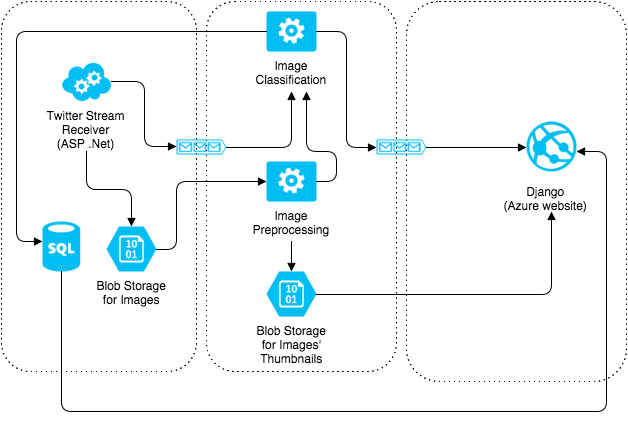
\includegraphics[width=35cm]
                           {../images/v1}
           \label{fig:desc}
           %% Figure
         \end{tikzfigure}

       }

       \block[
         %% titleoffsety=-3cm,
         %% bodyoffsety=-3cm
       ]
           {Web interface (first version)}{
         \begin{tikzfigure}[]
           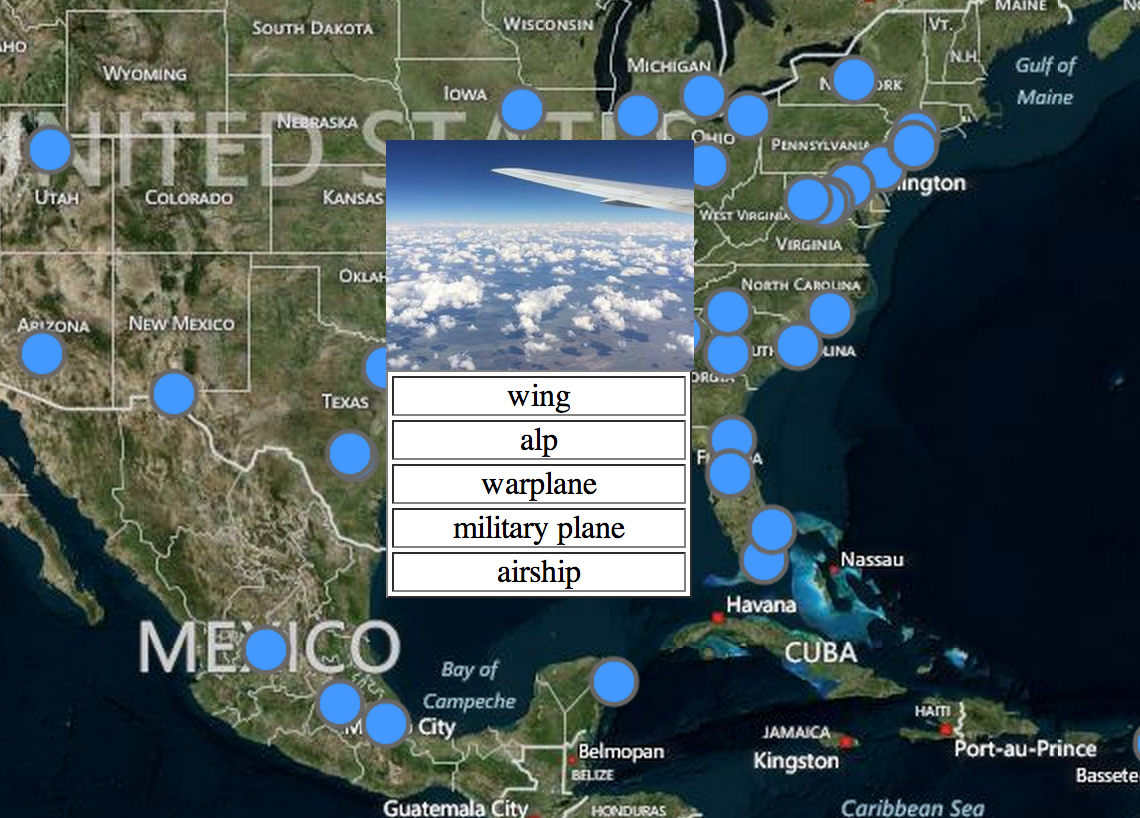
\includegraphics[height=13cm]
                           {../images/airplane}
           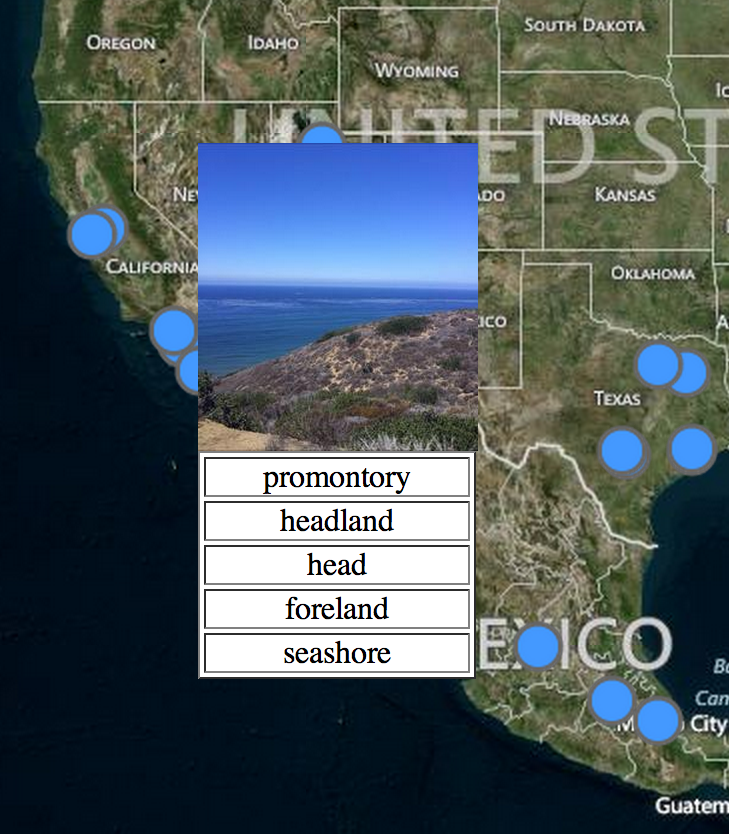
\includegraphics[height=13cm]
                           {../images/v1_promontory}
         \end{tikzfigure}

       }

      \block[
         %% titleoffsety=-5cm,
         %% bodyoffsety=-5cm,
       ]
       {Web interface (second version)}{
         \begin{tikzfigure}[]
           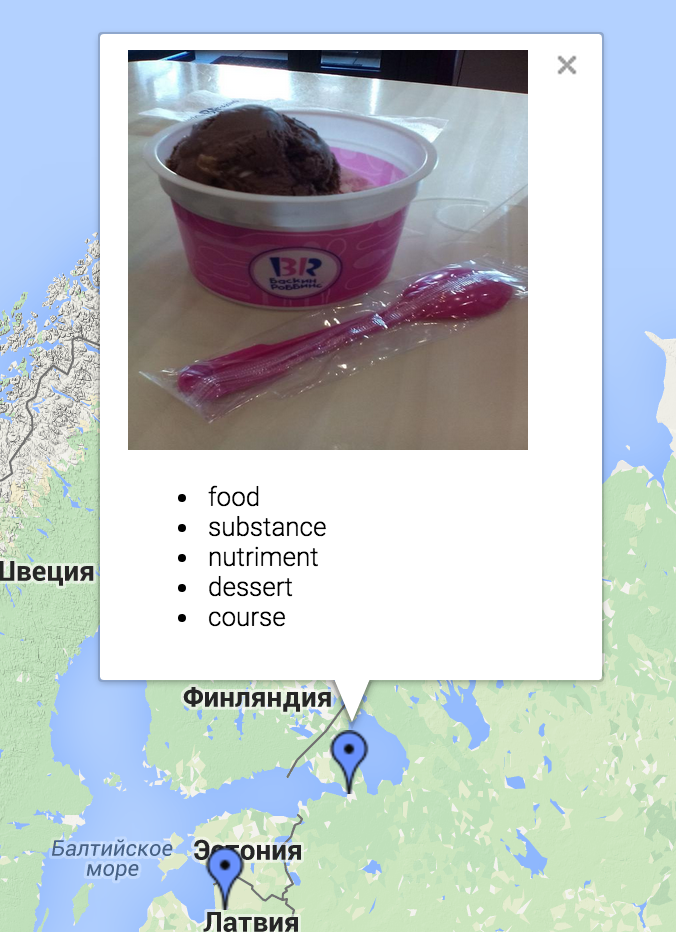
\includegraphics[height=13cm]
                           {../images/v2_food}
           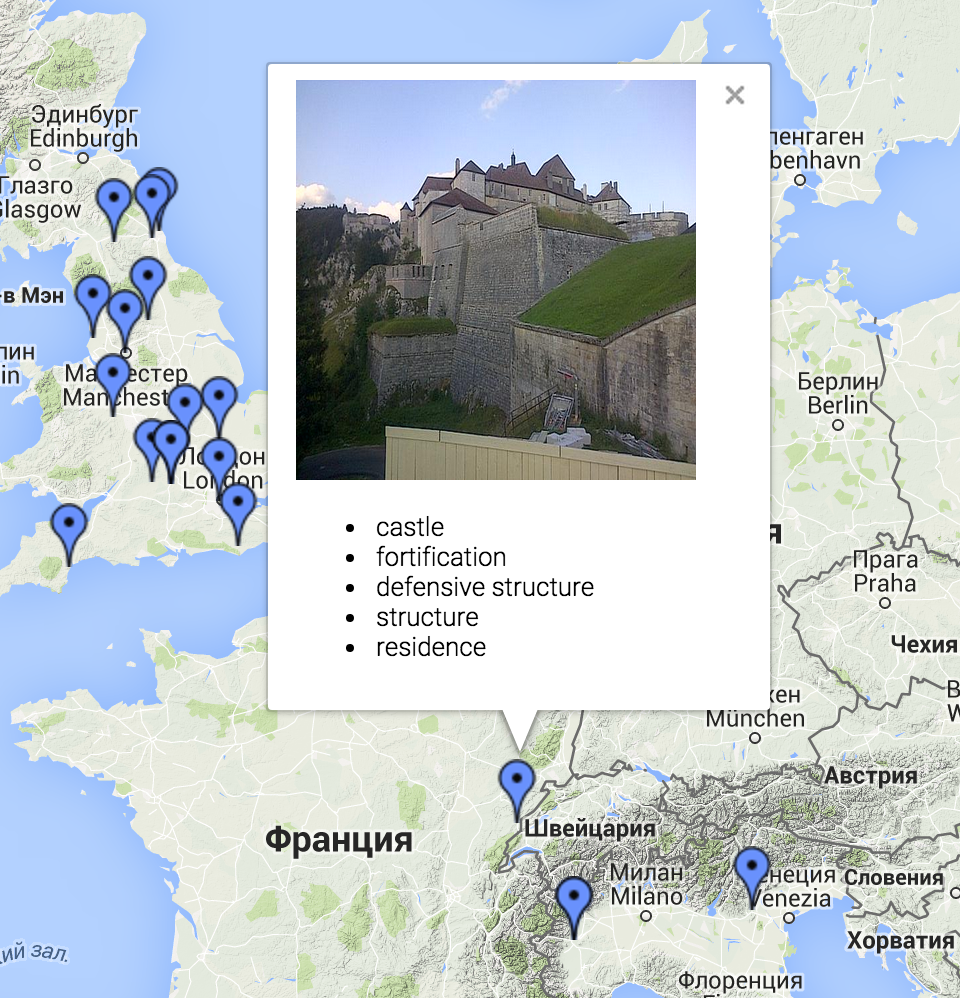
\includegraphics[height=13cm]
                           {../images/v2_castle}
           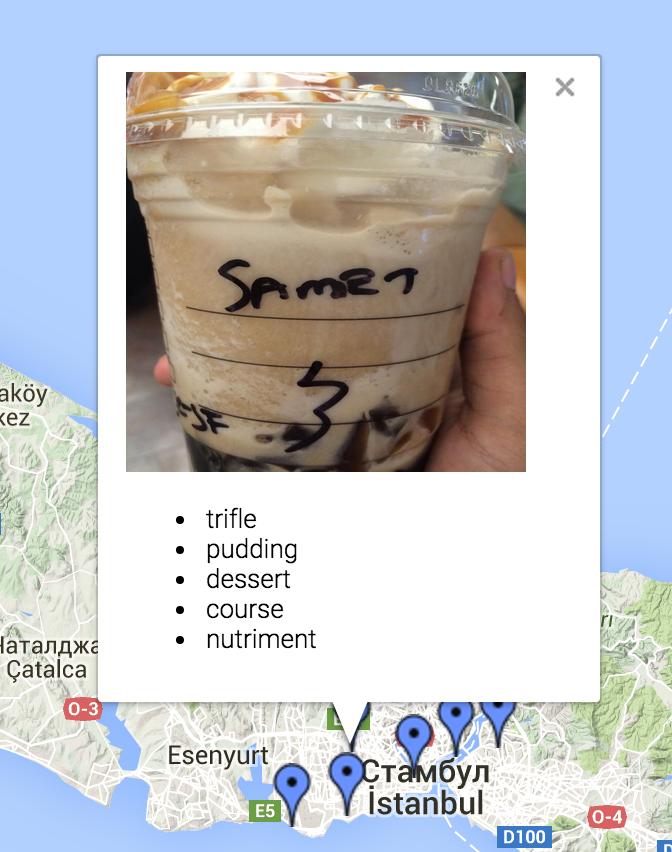
\includegraphics[height=13cm]
                           {../images/v2_trifle}
         \end{tikzfigure}

       }
       }
       \column{0.5}{
       \block[
         %% titleoffsety=-3cm,
         %% bodyoffsety=-3cm
       ]
           {Architecture of second version}{
         \begin{tikzfigure}[]
           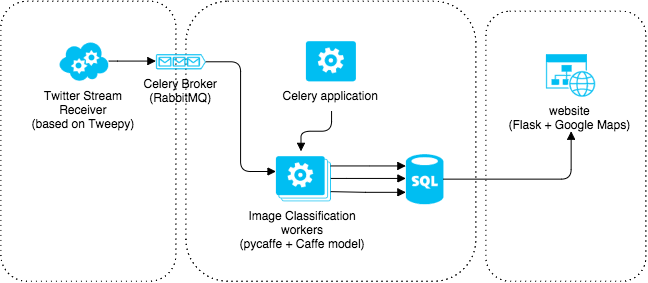
\includegraphics[width=35cm]
                           {../images/v2}
           \label{fig:desc}
         \end{tikzfigure}
       }
       \block[
         %% titleoffsety=-3cm,
         %% bodyoffsety=-3cm,
         %% titleoffsetx=3cm,
         %% bodyoffsetx=3cm,
         %% titlewidthscale=1.2,
         %% bodywidthscale=1.2,
       ]
       {Image classification}{
         A deep convolutional neural network was used as the classifier for images obtained from Twitter. Python library Caffe~\cite{caffe} with prebuilt Berkeley Vision and Learning Center (BVLC) CaffeNet Model were utilized. This model is a replication of an ImageNet model~\cite{nips2012} trained on the ILSVRC-2012 data set. It was released by BVLC for unrestricted use.

         Here is the short overview of the model: the best validation performance during training was on iteration 313,000 with validation accuracy 57.412\% and loss 1.82328.
This model obtains a top-1 accuracy 57.4\% and a top-5 accuracy 80.4\% on the validation set.
         Max-pooling layers follow first, second, and fifth convolutional layers.
         The number of neurons in each layer is given by 253440, 186624, 64896, 64896, 43264, 4096, 4096, 1000.~\cite{nips2012}

         \begin{tikzfigure}[]
           \includegraphics[width=35cm]
                           {../images/nips2012}
           \label{fig:desc}
           %% Figure
         \end{tikzfigure}

       }

       \block[
         %% titlewidthscale=.8,
         %% bodywidthscale=.8,
         %% titleoffsety=-26cm,
         %% bodyoffsety=-26cm,
         %% titleoffsetx=3cm,
         %% bodyoffsetx=3cm
       ]
         {References}{
         \renewcommand{\section}[2]{}%
         %\renewcommand{\chapter}[2]{}% for other classes
         %% \bibliographystyle{plain}
         \bibliography{poster}
       }
     }
     \end{columns}

 \end{document}
